\documentclass[14pt, a4paper]{extarticle}

%\usepackage[usenames,dvipsnames,svgnames,table]{xcolor}
\usepackage[
  a4paper, mag=1000, includefoot,
  left=3cm, right=1cm, top=2cm, bottom=2.5cm, headsep=1cm, footskip=1cm
]{geometry}

\usepackage{amsmath,amssymb,amsfonts}
\usepackage{mathtools}
\usepackage[cache=false,outputdir=.texpadtmp]{minted}
\usepackage{subcaption}
\usepackage{url}
\usepackage{svg}

\usepackage{polyglossia}
\setmainlanguage{russian} 
\setotherlanguage{english}
\newfontfamily\russianfont[Script=Cyrillic]{Times New Roman}
\newfontfamily{\cyrillicfonttt}{CMU Typewriter Text}

\linespread{1.5} % межстрочный интервал 

% Macro: Absolute value
\DeclarePairedDelimiter{\abs}{\lvert}{\rvert}
\DeclarePairedDelimiter{\norm}{\lvert\lvert}{\rvert\lvert}


\begin{document}

%-----------------------------------------
% Титульный лист
\thispagestyle{empty}

\begin{center}

\scriptsize{
Министерство образования и науки Российской Федерации

Федеральное государственное автономное образовательное учреждение высшего профессионального образования \\
}
\small{
\textbf{«Уральский федеральный университет} \\
\textbf{имени первого Президента России Б.Н. Ельцина»} \\
}
\normalsize{
\textbf{Институт математики и компьютерных наук} \\
\textbf{Кафедра алгебры и дискретной математики}
}

\vfill
\vfill

\Large О фильтрации событий в физике высоких энергий с помощью нейросетей с инверсией градиента.

\end{center}

\vfill

\begin{tabular}{cc}
{
\begin{minipage}[]{180pt}
«Допустить к защите»\\
\line(1,0){116} \\
\line(1,0){116} \\
«\line(1,0){16}»\ \line(1,0){84}\  2016 г.
\end{minipage}
} &
\begin{minipage}[]{240pt}
Выпускная квалификационная работа\\
студента 4 курса\\
Киселева Антона Ивановича\\  \newline
Научный руководитель:\\
кандидат физико-математических наук,\\
доцент КАДМ ИМКН УрФУ,\\
Клепинин Александр Владимирович\\
\end{minipage}
\end{tabular}

\vfill
\vfill

\begin{center}
Екатеринбург

2016
\end{center}

\sloppy

%-----------------------------------------
% Реферат
\newpage

\setcounter{page}{1}
\thispagestyle{empty}

\centerline{\large \textbf{Реферат}}

\bigskip
\bigskip

\noindent
Ключевые слова: доменная адаптация, глубокие нейронные сети, слой обращения градиента.

\medskip 

\noindent
Объект исследования~— доменная адаптация глубоких нейронных сетей.

\medskip 

\noindent
Цель работы~— рассмотреть применение способных к доменной адаптации нейронных сетей в задаче фильтрации событий.

\medskip 

\noindent
Результаты работы: разработана архитектура нейросети со слоем обращения градиента для данной задачи; проведены эксперименты для сравнения такой архитектуры с классической; сделан вывод по практической применимости подобной архитектуры в задаче фильтрации событий.

%-----------------------------------------
% Оглавление
\newpage

\tableofcontents

%-----------------------------------------
% Введение
\newpage

\addtocontents{toc}{\protect{\contentsline{section}{\numberline{}{Введение}}{\thepage}}}
\section*{Введение}

В современном мире каждый день создается невероятное количество информации. С одной стороны, люди общаются друг с другом через социальные сети и создают таким образом миллионы текстов. С другой стороны, есть миллионы устройств, которые собирают данные — шагомеры, приборы учета, видеокамеры, погодные станции и другие аналогичные устройства, регулярно получающие данные без значительного внимания людей. Анализ этих данных является крайне популярной на сегодняшний день темой. Она актуальна как в исследовательской среде, так и среди бизнеса. 

Анализ данных требует использования различных методов машинного обучения, таких как машины опорных векторов, решающие деревья или нейронные сети. Для большинства из этих методов наличие большого объема данных позволяет строить более точные модели. 

Одной из важных задач машинного обучения является задача классификации. К сожалению, для многих задач, сводящихся к задаче классификации, невозможно получить необходимый для получения хорошей модели объем данных. Это может быть связано как с тем, что для получения большого количества данных требуется затратить множество ресурсов, так и с тем, что генерирующие их процессы случаются довольно редко. Помимо этого, может быть такая ситуация, что достоверность данных сомнительна.

Одной из таких задач является поиск лептонных распадов, не сохраняющих лептонный аромат \cite{kaggle}. В Стандартной модели — общепринятой на данный момент модели физики элементарных частиц — считается, что аромат лептонов является физической характеристикой, которая сохраняется при распадах. В некоторых моделях физики элементарных частиц ароматы лептонов таким свойством не обладают. Успешное нахождение такого рода распадов откроет новые горизонты для физики элементарных частиц. Одним из таких распадов является распад $\tau^-\rightarrow\mu^+ \mu^- \mu^-$, данные которого рассмотрены в работе. Формальное определение задачи дано в параграфе \ref{paragraph:task}.

Одной из наиболее точных моделей, использующейся в задаче классификации, являются глубокие нейронные сети. Их устройство описано в параграфе \ref{paragraph:theory}. Во многих задачах классификации применение глубоких нейронных сетей с архитектурой прямого распространения сигнала дает хорошие результаты. К сожалению, на данный момент эти задачи ограничиваются лишь такими, для которых имеется большое количество размеченных данных для обучения.
Однако, для решения некоторых задач возможно получить дополнительный объем данных, которые будут отличаться от исходных, однако будут отвечать той же самой задаче. В таком случае исходные данные называются исходным доменом, а дополнительные данные целевым доменом. Возникает задача проведения доменной адаптации — получения такого классификатора, который бы успешно проводил классификацию вне зависимости от того, из какого домена ему был предоставлен вход. Важным примером таких задач являются задачи, для которых возможно получить множество размеченных синтетических данных с одной стороны и неразмеченных реальных данных с другой.

Одним из методов проведения доменной адаптации является предложенная в \cite{ganin} архитектура нейронной сети. Она состоит из трех частей — экстрактора признаков и параллельно подключенных к нему классификаторов класса и классификаторов домена, последний подключен через так называемый слой обращения градиента. Это позволяет ему при обучении помогать экстрактору признаков выделять именно такие признаки, которые не различают исходный и целевой домены между собой. Подробней архитектура описана в параграфе \ref{paragraph:method}.

В рамках исследования была построена нейросетевая архитектура прямого распространения сигнала описанного выше типа для задачи фильтрации в физике высоких энергий. Помимо этого, рассмотренная архитектура была реализована в виде программы на языке Python. Были предложены две новых методики обучения такой архитектуры. Все вышесказанное предложено в параграфе \ref{paragraph:architecture}.

В параграфе \ref{paragraph:results} приведены экспериментальные результаты проверки предложенных методик, а в параграфе \ref{paragraph:analysis} проведен их анализ.

Было выяснено, что одна из методик обучения не дает желаемый результат, в то же время как другая демонстрирует действенность применения нейросетевой архитектуры со слоем обращения градиента в исследуемой задаче.

\newpage 

%-------------------------------------------------------
% Теория
\section{Теоретический материал}
\label{paragraph:theory}

В этом параграфе дается формальное определение задачи классификации, а так же вводится понятие доменной адаптации. Дополнительно, напомнены основные факты о внутреннем устройстве нейронной сети, а также описаны используемые в дальнейшем элементы нейросетевой архитектуры.

\subsection*{Задача классификации}
\label{class_task}

Рассмотрим задачу классификации из многомерного пространства $X$ в конечное пространство меток $Y$. Пусть нам даны ${x_1, x_2, ..., x_N}$ — обучающая выборка, где $x_i \in X$. Для каждого $x_i$ нам известно значение метки $y_i$, при этом $y_i \in Y$. Требуется построить такой оператор $H(x): X \rightarrow Y$, который как можно более точно предсказывает метки для каждого нового $x \in X$. Такой оператор далее называется классификатором.

Усложним постановку задачи. Предположим, что пространство $X$ разделяется на два непересекающихся множества $S$ и $T$. Для каждого $x_i$ из обучающей выборки справедливо следующее: если $x_i \in S$, соответствующая ему метка $y_i$ известна; если же $x_i \in T$, то эта метка неизвестна. Для простоты записи, поставим в соответствие таким записям символ $\mathbb{?}$. Далее $S$ и $T$ называются исходным и целевым доменами. Также, будем использовать следующее обозначение:
\begin{equation*}
	d_i = 0 \Leftrightarrow x_i \in S \quad \quad \quad
	d_i = 1 \Leftrightarrow x_i \in T 
\end{equation*}
Другими словами, эта задача классификации сводится к предыдущей, у которой пространство меток $Y^{'} = Y \cup \{?\}$.

 Построение классификатора, который бы предсказывал по элементу $x \in X$ соответствующую ему метку $y \in Y$ при условии обучения на обучающей выборке $\{(x_1, y_1), ... (x_N, y_N)\}$, где метки $y_i$ известны лишь для элементов $x_i \in S$ (иначе $x_i \in T$ и  $y_i =~?$), называется доменной адаптацией. В результате этого процесса от классификатора требуется предъявлять метку $y \in Y$ для любого $x \in X$ вне зависимости от того, какому домену он принадлежит, то есть он должен не различать два домена — исходный и целевой — между собой. 

\subsection*{Устройство нейронной сети}

В этом пункте приведены базовые понятия, используемые для проектирования нейронных сетей. Помимо этого, даны описания используемых далее элементов архитектуры нейросети. Более подробное описание дано в \cite{deep_learning} и в \cite{haykin}.

Перед тем, как описать устройство нейронной сети, напомним понятие \textit{нейрона}. Нейроном называется функция $h_{w, b}(x): \mathbb{R}^{n} \rightarrow \mathbb{R}$:

\begin{equation*}
	h_{w, b}(x) = f(w^Tx) = f(\sum_i w_ix_i + b)
\end{equation*}
\begin{itemize}
\item $f: \mathbb{R} \rightarrow \mathbb{R} $ — функция активации нейрона;
\item $w \in \mathbb{R}$ — вектор весов нейрона;
\item $w_i \in \mathbb{R} $ — весовые коэффициенты нейрона;
\item $b$ — коэффициент смещения.
\end{itemize}

Таким образом один слой в нейронной сети можно описать как функцию $h_{W, B}: R^n \rightarrow R^m$ из $m$ определенных выше функций, где $W$ — матрица весов слоя, строки которой являются векторами весов соответствующих нейронов. Удобно считать, что у нейрона есть еще один коэффициент на вход, который всегда равен единице — его вес обозначается $b$. Сама сеть состоит из подобных слоев таким образом, что выход одного слоя является входом для другого. 

Классической архитектурой для нейронных сетей является архитектура прямого распространения сигнала. В такой архитектуре слои подключены друг к другу без циклов. Рассмотрим такую архитектуру на примере трехслойной нейросети:
\begin{center}
	\includegraphics[scale=0.3]{images/network_example.png}
\end{center}

\begin{equation*}
	a^{(2)} = f(W^{(2)}x + b^{(2)})
\end{equation*}
\begin{equation*}
	h_{W, b}(x) = f(W^{(3)}a^{(2)} + b^{(3)})
\end{equation*}
\begin{itemize}
\item Под применением функции активации к вектору подразумевается ее покоординатное применение.
\item $W^{(i)}, b^{(i)}$ — матрица весов и вектор смещений слоя $i$;
\end{itemize}

Приведенные выше уравнения называются \textit{прямым распространением сигнала}. Итоговый выход $h_{W, b}(x)$ получается последовательным умножением выхода предыдущего слоя на матрицу весов текущего слоя, а также дальнейшим покоординатным применением функции активации. Обобщим данные уравнения на случай произвольного количества последовательно подключенных слоев:
\begin{equation*}
	a^{(0)} = x
\end{equation*}
\begin{equation*}
	a^{(l+1)} = f(W^{(l+1)}a^{(l)} + b^{(l+1)})
\end{equation*}
\begin{itemize}
	\item $l$ — номер слоя.
\end{itemize}

\subsection*{Обучение нейронной сети}
Пусть $\{(x^{(1)}, y^{(1)}), ..., (x^{(N)}, y^{(N)})\}$ — обучающая выборка из $N$ элементов. Под обучением подразумевается минимизация функции ошибки на элементах обучающей выборки. Она производится при помощи метода градиентного спуска. Проведем дальнейшие рассуждения, используя функцию квадратичную функцию потерь $E(W, b)$:

\begin{equation*}
	E(W, b; x, y) = \frac{1}{2} \norm{h_{W,b}(x)-y}^2
\end{equation*}
\begin{itemize}
	\item $(x, y)$ — элемент выборки;
	\item $h_{W,b}(x)$ — представление всей нейронной сети как функции от входа $x$;
	\item $W, b$ — весовые коэффициенты и коэффициенты смещений для всех слоев нейронной сети.
\end{itemize}
Для всей обучающей выборки она примет вид:
\begin{equation*}
	E(W, b) = \frac{1}{m} \sum^{m}_{i=1} E(W, b; x^{(i)}, y^{(i)})
\end{equation*}
Целью обучения является минимизация функции потерь. В соответствии с методом градиентного спуска уравнения оптимизации выглядят следующим образом:
\begin{equation*}
	W^{(l)}_{ij} := W^{(l)}_{ij} - \alpha \frac{\partial}{\partial W^{(l)}_{ij}} E(W, b)
\end{equation*}
\begin{equation*}
	b^{(l)}_i := b^{(l)}_i- \alpha \frac{\partial}{\partial b^{(l)}_i} E(W, b),
\end{equation*}
\begin{itemize}
	\item $l$ — номер слоя;
	\item $W^{(l)}_{ij}$, $b_i$ — коэффициенты матрицы слоев и вектора смещений слоя $l$;
	\item $\alpha$ — коэффициент скорости обучения (learning rate).
\end{itemize}
Заметим, что:
\begin{equation*}
	\frac{\partial}{\partial W^{(l)}_{ij}} E(W, b) = \frac{1}{m} \sum^m_{i=1} \frac{\partial}{\partial W^{(l)}_{ij}} E(W, b; x^{(i)}, y^{(i)})
\end{equation*}
\begin{equation*}
	\frac{\partial}{\partial b^{(l)}_i} E(W, b) = \frac{1}{m} \sum^m_{i=1} \frac{\partial}{\partial b^{(l)}_i} E(W, b; x^{(i)}, y^{(i)})
\end{equation*}

Каждый из параметров $W^{(l)}_{ij}$ и $b^{(l)}_i$ инициализируется различными случайными близкими к нулю значениями. Это требуется для того, чтобы нейроны обучились различным функциям.

Для распространения градиентного спуска по весам всей сети используется алгоритм обратного распространения ошибки. Он приведен ниже.

Для простоты записи, введем следующее обозначение:
\begin{equation*}
	a, b, c\in \mathbb{R}^n, a \bullet b = c \Leftrightarrow \forall i = 1, 2, ..., n: a_i b_i = c_i
\end{equation*}
Другими словами, символ $\bullet$ обозначает покоординатное умножение координат двух векторов.

В таких обозначениях алгоритм обратного распространения ошибки имеет следующий вид:
\begin{enumerate}
	\item Произведем прямое распространение сигнала по сети через все слои \\ $L_1$, ..., $L_{n_l}$.
	\item Для выходного слоя $n_l$ посчитаем: \\ $\delta^{(n_l)} = - (y - a^{(n_l)}) \bullet f'(z^{(n_l)})$
	\item Для остальных слоев $l = n_1-1, ..., 2$: \\ $\delta^{(l)} = ((W^{(l)})^T\delta^{(l+1)}) \bullet f'(z^{(l)})$
	\item Вычислим необходимые производные: \\ $\nabla_{W_{l}} E(W, b; x, y) = \delta^{(l+1)}(a^{(l)})^T$ \\ $\nabla_{b_{l}} E(W, b; x, y) = \delta^{(l+1)}$ \\ $\nabla_{W_{l}}E$, $\nabla_{W_{b_l}}E$ — градиент функции потерь по весам и по коэффициенту смещения слоя $l$.
\end{enumerate}

В результате метод градиентного спуска примет следующий вид:
\begin{enumerate}
	\item $\Delta W^{(l)} := 0$, $\Delta b^{(l)} := 0$ — смещения параметров каждого слоя, вычисляемые в дальнейшем.
	\item Для $i = 1, 2, ..., m$:
	\begin{enumerate}
	\item Вычисляем $\nabla_{W_{l}} E(W, b; x, y), \nabla_{b_{l}} E(W, b; x, y)$ через алгоритм обратного распространения ошибки.
	\item $\Delta W^{(l)} := \Delta W^{(l)} + \nabla_{W_{l}} E(W, b; x, y)$
	\item $\Delta b^{(l)} := \Delta b^{(l)}  + \nabla_{b_{l}} E(W, b; x, y)$
	\end{enumerate}
	\item Обновляем параметры: \\ $W^{(l)} := W^{(l)} - \alpha (\frac{1}{N} \Delta W^{(l)})$ \\ $b^{(l)} := b^{(l)} - \alpha (\frac{1}{N} \Delta b^{(l)})$
\end{enumerate}

Каждое исполнение шагов 1-3 в алгоритме выше называется \textit{эпохой}. Их количество произвольно.

Как можно заметить в алгоритме для метода градиентного спуска, в шаге 2 алгоритм обратного распространения ошибки вычисляется для каждого элемента из обучающей выборки. К сожалению, применение методов, использующих всю выборку, отнимает слишком много вычислительных ресурсов в случае большой обучающей выборки. Поэтому на практике и далее использован стохастический градиентный спуск. Этот метод вместо использования всей выборки случайным образом делит выборку на подвыборки, и в рамках каждой эпохи выполняет весь алгоритм для них. С одной стороны, как отмечено в \cite{sgd}, при таком проведении процедуры каждое обновление будет малым, а следовательно в некоторых случаях это может обеспечить более стабильную сходимость. С другой стороны, так как вычисления подобного рода являются матричными, их вычисление возможно оптимизировать и вычислять на специализированных устройствах, разработанных для быстрого выполнения операций для небольших матриц. Одними из таких устройств являются видеокарты.

\subsection*{Слой Dropout}
В работе \cite{dropout} был предложен dropout-слой как средство регуляризации. Он работает следующим образом: во время обучения нейрон такого слоя присутствует в модели с фиксированной вероятностью $p$; во время же использования модели он присутствует всегда, однако его вес умножается на $p$. Наглядно это изображено на рис. \ref{figure:dropout}.

\begin{figure*}
\begin{subfigure}{.5\textwidth}
	\centering
	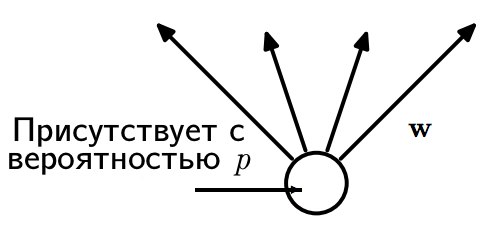
\includegraphics[scale=.85]{images/dropout1.png}
	\caption{Поведение слоя Dropout во время обучения}
\end{subfigure}
\begin{subfigure}{.5\textwidth}
	\centering
	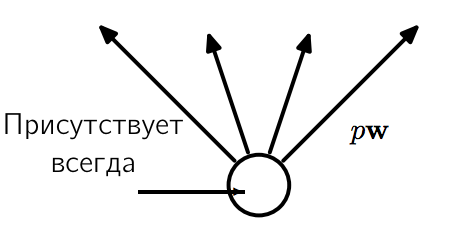
\includegraphics[scale=.9]{images/dropout2.png}
	\caption{Поведения слоя Dropout во время использования модели}
\end{subfigure}
\caption{Диаграмма поведения слоя Dropout во время различных режимов работы нейронной сети}
\label{figure:dropout}
\end{figure*}

Добавление таких слоев в модель помогает избежать переобучения — такое ограничение на строение нейросети способствует обучению особенностям обучающей выборки всей нейросети в целом, а не каждого конкретного нейрона. Помимо этого, на такой прием можно посмотреть как на совмещение нескольких нейросетевых классификаторов в одной нейросети. Как отмечают авторы работы, такой подход показывает наилучшие на данный момент результаты в задаче распознавания изображений.

\subsection*{Функция активации PReLU}
В статье \cite{prelu} предлагается кусочно-линейная функция активации, под названием PReLU. Она определяется следующим образом:

\begin{figure*}
\begin{center}
	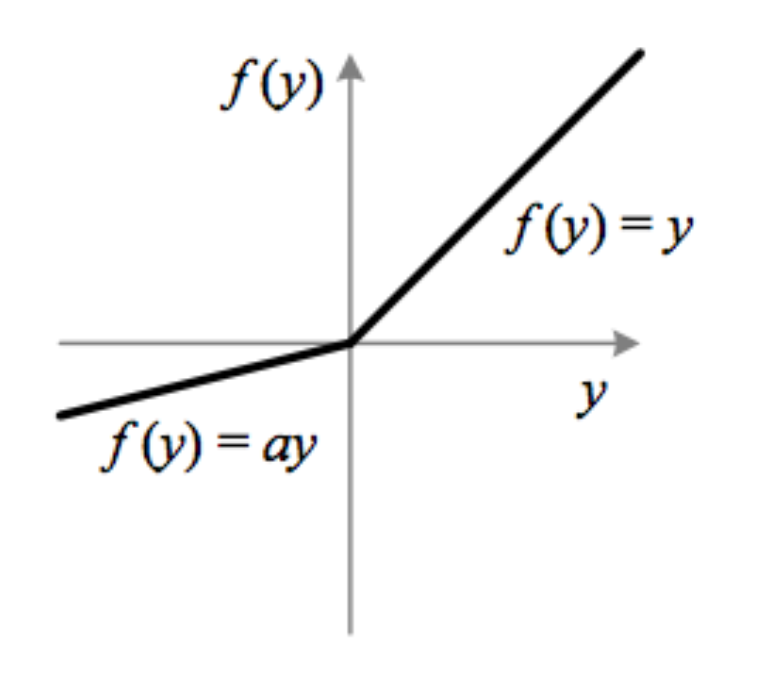
\includegraphics[scale=0.4]{images/prelu.png}
\end{center}
	\caption{График функции активации PReLU}
	\label{figure:prelu}
\end{figure*}

\begin{equation*}
	f(y_i) = \begin{cases}
		y_i, & \text{при $y_i \geq 0$} \\
		a_iy_y, & \text{при $y_i < 0$}
	\end{cases}
\end{equation*}

График функции PReLU приведен на рис. \ref{figure:prelu}. Заметим, что параметр $a_i$ уникален для каждой координаты вектора $y$. Эти коэффициенты близки к нулю и подбираются в процессе обучения. 
Авторы утверждают, что такая функция активации улучшает результат функции активации ReLU: $f(x) = max(0, x)$. Аналогичные результаты получили и авторы \cite{prelu_experiment}.

\newpage

%-------------------------------------------------------
% Исследуемая архитектура нейронной сети
\newpage
\section{Исследуемая архитектура нейронной сети}
\label{paragraph:method}
 
В этом параграфе описана предложенная в \cite{ganin} архитектура нейронной сети. 

Рассмотрим задачу классификации, рассмотренную в параграфе \ref{paragraph:theory}. Для ее решения в \cite{ganin} предлагается применить следующую архитектуру нейронной сети. Она представима в виде трех сегментов, наглядно показанных на рис. \ref{figure:architecture}.
 
\begin{figure*}
	\includegraphics[scale=0.58]{images/grl_architecture1.png}
	\caption{Исследуемая архитектура нейронной сети}
	\label{figure:architecture}
\end{figure*}
 
Первый из сегментов называется \textit{экстрактором признаков} и обозначается как $G_d$. Он занимается тем, что по исходному входу $x \in X$ возвращает вектор $f \in \mathbb{R}^D$. Если обозначить за $\theta_f$ параметры всех слоев экстрактора, то результат использования экстрактора признаков записывается следующим образом:
\begin{equation*}
	 f = G_d(x, \theta_d)
\end{equation*}
 
Второй сегмент продолжает первый и называется \textit{классификатором класса}. Его обозначение: $G_y$. Он по выданным $G_f$ признакам $f$ возвращает метку $y$. Параметры всех его слоев обозначены как $\theta_y$. Для классификатора класса используется следующее аналогичное обозначение:
\begin{equation*}
	y = G_y(f, \theta_y)
\end{equation*}
 
Третий сегмент $G_d$ также продолжает экстрактор признаков и возвращает метку домена $d$. Его название — \textit{классификатор домена}. Он имеет параметры $\theta_d$.
\begin{equation*}
	d = G_d(f, \theta_d)
\end{equation*}

Поставим перед нейронной сетью цель — проведение доменной адаптации через процедуру обучения.
Для данной архитектуры это означает получение таких признаков $f$, для которых домены, порожденные экстрактором признаков из исходных доменов, будут схожи. Другими словами, требуется:
\begin{itemize}
	\item рассмотреть признаки $f$ как элементы пространства $F$;
	\item перейти от исходных признаков $x \in X$ к новым признакам $f \in F$ при помощи экстрактора признаков $G_f$;
	\item в $F$ рассмотреть домены $S(f) = \{G_f(x; \theta_f)~|~x \in S \}$ и $T(f) = \{G_f(x; \theta_f)~|~x~\in~T\}$;
	\item обучить $G_f$ таким образом, чтобы он не различал между собой эти два домена.
\end{itemize}

Для выполнения вышеизложенного авторы \cite{ganin} рассматривают следующий функционал:

\begin{equation*}
\begin{gathered}
E(\theta_f, \theta_y, \theta_d) = \\ \sum_{ \substack{i=1..N \\ d_i=0} }L_y(G_y(G_f(x_i; \theta_f); \theta_y), y_i) - \lambda \sum_{ i=1..N } L_d(G_d(G_f(x_i; \theta_f); \theta_d), y_i) = \\\sum_{ \substack{i=1..N \\ d_i=0} } L_y^i(\theta_f, \theta_y) - \lambda \sum_{ i=1..N }  L_d^i(\theta_f, \theta_d)
\end{gathered}
\end{equation*}
\begin{itemize}
\item $L_y(·, ·)$ —~ функция потерь классификатора класса;
\item $L_d(·, ·)$ —~ функция потерь классификатора домена;
\item $\lambda$ —~ параметр, контролирующий компромис между уменьшением первого слагаемого и увеличением второго.
\end{itemize}

Далее, производится поиск параметров $\hat \theta_f, \hat \theta_y, \hat \theta_d$, образующих седловую точку функционала:

\begin{equation*}
	(\hat \theta_f, \hat \theta_d) = \text{arg}~\underset{\theta_f, \theta_d}{\text{min}}~E(\theta_f, \theta_y, \hat \theta_d)
\end{equation*}
\begin{equation*}
	\hat \theta_d = \text{arg}~\underset{\theta_d}{\text{max}}~E(\hat \theta_f, \hat \theta_y, \theta_d)
\end{equation*}

Поиск параметров осуществляется при помощи алгоритма градиентного спуска. Обновления параметров в алгоритме для такого функционала имеют следующий вид:

\begin{equation*}
\begin{split}
	\theta_f \leftarrow \theta_f - \mu \Bigg( \frac{\partial L^i_y}{\partial \theta_f} - \lambda \frac{\partial L^i_d}{\partial \theta_f} \Bigg) \\
	\theta_y \quad \quad \leftarrow \quad \theta_y - \mu \frac{\partial L^i_y}{\partial \theta_y} \\
	\theta_d \quad \quad \leftarrow \quad \theta_d - \mu \frac{\partial L^i_d}{\partial \theta_d} 
\end{split}
\end{equation*}
\begin{itemize}
	\item $\mu$ — коэффициент скорости обучения.
\end{itemize}

При таких параметрах с одной стороны достигается минимум функции потерь для классификатора класса $G_y$, а с другой максимум для функции потерь классификатора домена $G_d$. Это обеспечивает формирование признаков $f$ как оптимально различающими классы c одной стороны, так и независимыми от домена с другой.

Для обеспечения такого поведения произведено следующее: классификатор домена $G_d$ подвлючен к экстрактору признаков $G_d$ через специальный \textit{слой обращения градиента}. Его действие описывается в терминах псевдо-функции $R_{\lambda}$:
\begin{equation*}
	R_{\lambda}(x) = x \quad \quad \quad \quad
	\frac{dR_{\lambda}}{dx} = -\lambda I, \text{где $I$ — единичная матрица}
\end{equation*}
\begin{itemize}
	\item $\lambda$ — параметр слоя, на который умножаются градиенты функции потерь в процедуре градиентного спуска.
\end{itemize}
В таких обозначениях подключение примет вид:
\begin{equation*}
\forall i = 1, ..., N: \quad \quad \quad \quad
f_i = G_f(x_i; \theta_f) \quad \quad \quad \quad
d_i = G_d(R_{\lambda}(f_i); \theta_d)	
\end{equation*}
\begin{itemize}
	\item $N$ — размер обучающей выборки.
\end{itemize}

Другими словам, при прямом распространении сигнала этот слой просто возвращает свой вход, а применение к этому слою оператора дифференцирования превращает его в оператор, умножающий вход на $-\lambda$. С его помощью определение описанного выше функционала переписывается следующим образом:

\begin{equation*}\label{E}
\begin{gathered}
E(\theta_f, \theta_y, \theta_d) = \\ \sum_{ \substack{i=1..N \\ d_i=0} }L_y(G_y(G_f(x_i; \theta_i); \theta_y), y_i) + \sum_{ i=1..N } L_d(G_d(R_{\lambda}(G_f(x_i; \theta_i)); \theta_d), y_i)
\end{gathered}
\end{equation*}

В итоге, нахождение минимума для этого функционала обеспечивает как оптимальное качество классификации, так и неразличимость доменов $S(f)$ и $T(f)$.

%-------------------------------------------------------
% Задача
\section{Задача}
\label{paragraph:task}

В этом параграфе формально описана задача, для которой расмотрено применение архитектуры со слоем обращения градиента.

Для исследования была выбрана задача из соревнования \cite{kaggle_contest} с сайта \texttt{kaggle.com}, проходившего с 20 июля по 12 октября 2015 года. Соревнующимся был дан набор данных, содержащий как синтетические, так и реальные данные из эксперимента LHCb Большого Адронного Коллайдера. По этим данным было предложено построить модель, которая сможет выявлять наличие событий, соответствующих распаду $\tau \rightarrow 3\mu$. Обнаружение таких событий будет означать нарушение предсказываемого Стандартной моделью свойства сохранения аромата у лептонов, которому данный распад не подчиняется. Более подробно про задачу написано в \cite{kaggle}.

В этом соревновании, помимо получения качественного классификатора, соревнующимся требуется чтобы этот классификатор удовлетворял дополнительным требованиям. Они приведены ниже.

\subsection*{Процедура проверки решения}

\subsubsection*{Проверка на согласованность}
\label{agreement_metrics}
Поскольку для обучения классификатора участникам были предоставлены как реальные, так и синтетические данные, при создании классификатора имела место возможность обучить классификатор следующим образом: вместо обучения физическим отличиям между сигналом и фоном классификатор обучается неточностям моделирования синтетических данных. С точки зрения проверки физических гипотез, использование таких классификаторов неприемлемо. 

Чтобы избежать использования в решении задачи таких классификаторов, при проверке решения используется критерий Колмогорова-Смирнова. Его значение далее называется показателем $KS$. Он рассчитывается следующим образом:
\begin{equation*}
	KS = max \abs{F_{simulation} - F_{real}}
\end{equation*}
\begin{itemize}
	\item $F_{simulation}, F_{real}$ — функции распределения для синтетических и реальных данных соответственно
\end{itemize}

Большее значение этого критерия будет означать большую зависимость между значениями классификатора на реальных и синтетических данных соответственно.
Для принятия проверочной системой решения требуется, чтобы $KS < 0.09$.


\subsubsection*{Проверка на корреляцию с массой}
\label{mass_metrics}
Помимо этого, полученный классификатор может в процессе обучения по предоставленным данным научиться восстанавливать массу исходной частицы, распад которой был зафиксирован. Такое поведение вызывает некорректную оценку фона и может привести к ложным обнаружениям сигнала. Классификаторам требовалось избегать таких обнаружений.

Для проверки классификатора на корреляцию с массой исходной частицы применяется критерий Крамера-Мизеса, описанный в \cite{cramer}. Для его вычисления функция распределения на всем диапазоне масс сравнивается с функцией распределения на некотором интервале. После этого итоговое значение для критерия усредняется по всем интервалам:

\begin{equation*}
	CvM_{interval} = \int (F_{global} - F_{local})^2 dF_{global},
\end{equation*}
\begin{equation*}
	CvM = \langle CvM_{interval} \rangle_{interval}
\end{equation*}
\begin{itemize}
	\item $F_{global}, F_{local}$ — функции распределения для всех данных и для данных в некотором интервале масс.
\end{itemize}
Далее значение этого критерия называется показателем $CvM$. Чтобы решение засчитывалось, в условии задачи требуется, чтобы $CvM < 0.002$.

\subsubsection*{Показатель качества}
Качество полученного в процессе состязания классификатора оценивается при помощи взвешенного показателя $AUC$ (в других источниках — AUROC, area under ROC curve). Этот показатель рассчитывается как площадь под ROC-кривой \cite{roc_wiki}, построенной для результатов классификатора на тестовой выборке.
Для построения ROC-кривой вычисляются два параметра: TPR (True Positive Rate) — чувствительность классификатора, FPR (False Positive Rate) — специфичность классификатора. Для простоты, два разделяемых классификатором класса называются истинным и ложным классами.
\begin{equation*}
	TPR = \frac{TP}{TP + FN}, FRP = \frac{FP}{FP+TN}
\end{equation*}
\begin{itemize}
	\item $TP$ — количество верно положительных ответов классификатора;
	\item $FN$ — количество ложно отрицательных ответов классификатора (он указывает на ложный класс, а на самом деле класс истинный);
	\item $FP$ — количество ложно положительных ответов;
	\item $TN$ — количество верно отрицательных ответов.
\end{itemize}
Для построения кривой показатели TPR и FPR вычисляются для различных порогов бинаризации результатов классификатора (например, 0.01, 0.02 и так далее). Показатель $AUC$ считается как площадь под ROC-кривой. 
В данном конкретной задаче показатель $AUC$ отличается от общепринятого и называется weighted $AUC$. Его отличие в том, что вклад площади конкретных сегментов под ROC-кривой в показатель $AUC$ различен и показан показан на рис. \ref{figure:auc}. Для простоты в дальнейших рассуждениях он по прежнему указан как $AUC$.

\begin{figure}
	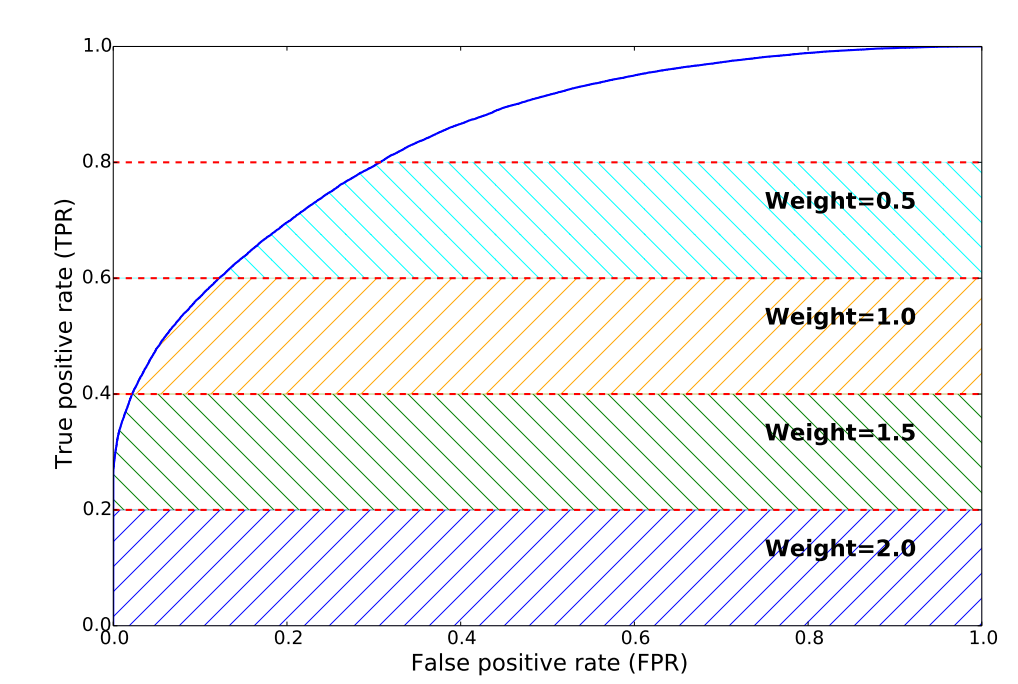
\includegraphics[scale=0.85]{auc.png}
	\caption{ROC-кривая. По горизонтали — показатель TPR, по вертикали — FPR.}
	\label{figure:auc}
\end{figure}


\subsection*{Формат данных}
Для анализа участникам состязания предоставлены четыре файла:
\begin{enumerate}
\item \texttt{training.csv} — набор размеченных данных для обучения классификатора, целевой переменной является переменная \texttt{signal}. События с  \texttt{signal = 1} являются сигналом, \texttt{signal = 0} — фоном. Стоит заметить, что все события сигнала являются синтетическими, а все фоновые события — реальными.
\item \texttt{check\_agreement.csv} — набор размеченных данных для проверки на согласованость. Признаки такие же, как и в \texttt{training.csv}, в том числе \texttt{signal} отвечает за домен — \texttt{signal = 1} для синтетических данных и \texttt{signal = 0} для реальных. 
\item \texttt{check\_correlation.csv} — набор данных для проверки классификатора на коррелированность с массой. Включает дополнительный признак \texttt{mass}, с которым проверяется результатов классификатора при помощи показателя $CvM$.
\item \texttt{test.csv} — набор неразмеченных тестовых данных, для которых участникам необходимо предоставить метки классов.
\end{enumerate}

%-------------------------------------------------------
% Применение архитектуры к задаче
\section{Применение архитектуры к задаче}
\label{paragraph:architecture}

В этом параграфе формализована постановка задачи классификации по отношению к исследуемой задаче, описана экспериментально исследуемая архитектура нейронной сети, показана ее реализация на языке программирования, а также описаны три процесса обучения нейросетевого классификатора. Помимо этого, приведена методика численного эксперимента для сравнения этих процессов.

\subsection*{Спецификация задачи}

В исследуемой задаче предоставлен набор данных для обучения \texttt{training.csv}. Напомним, что целевой переменной в задаче является переменная \texttt{signal}. Таким образом, перед нами стоит задача классификации, у которой $Y = \{0, 1\}$. Другое название этой задачи — бинарная задача классификации (всего два класса), или же задача фильтрации (под $1$ и $0$ подразумевается удовлетворение или нет какому-либо критерию). 

Стоит заметить, что все события сигнала являются синтетическими, а все фоновые события — реальными. Таким образом данные обучающей выборки разделяются на два домена:
\begin{equation*}
	S = \{ x \in X~|~signal(x) = 1 \} \quad \quad \quad
	T = \{ x \in X~|~signal(x) = 0 \} \quad \quad \quad
\end{equation*}
\begin{itemize}
	\item $signal(x)$ — значение целевой переменной \texttt{signal} для элемента $x$ обучающей выборки.
\end{itemize}

Заметим, что данная постановка не вполне соответствует данной в параграфе \ref{paragraph:theory} постановке усложненной задачи классификации — для нас известно значение целевой переменной для элементов из целевого домена $T$. Отметим, что проверка на соответствие требует от классификатора слабо различать эти два домена между собой.

К счастью, устройство исследуемой архитектуры нейронной сети способствует выделению именно таких признаков, которые не позволяют различить эти два домена. Таким образом, само строение нейронной сети способствует удовлетворению требуемых в задаче условий соответствия.

\subsection*{Описание использованной нейросетевой архитектуры}

Для исследования метода было выбрано строение нейронной сети, показанное на рис. \ref{fig:neural_net}. На нем используются следующих обозначения:

\begin{figure*}
	\centering
	\includegraphics[scale=0.45]{images/model.pdf}
	\caption{Диаграмма разработанной архитектуры}
	\label{fig:neural_net}
\end{figure*}

\begin{itemize}
	\item \textit{Dense($n$)}: слой из $n$ нейронов, каждый из которых соединен с выходом каждого нейрона из предыдущего слоя;
	\item \textit{Dropout($p$)}: слой Dropout с параметром вероятности равным $p$;
	\item \textit{PReLU}: слой, осуществляющий функцию активации PReLU;
	\item \textit{GradientReversal}: слой обращения градиента;
	\item \textit{Softmax}: слой с функцией активации, осуществляющий функцию мягкого максимума \\ $f(x)_j = \frac{e^{x_j}}{\sum_{k=1}^K e^{x_k}}, \text{где~} K \in \mathbb{N} \text{ — размерность входа}, x \in \mathbb{R}^K, j=1,2,..., K$;
	\item $input\_size$ — количество признаков, подаваемых классификатору на вход;
	\item $Feature Extractor$, $Label Classifier$, $Domain Classifier$ — экстрактор признаков, классификатор класса и классификатор домена соответственно.
\end{itemize}

Глобально данная архитектура соответсвует описанной в параграфе \ref{paragraph:method}. Каждый конкретный сегмент рассматривается как классическая нейронная сеть с прямым распространением сигнала. Слои Dropout между полностью соединенными слоями играют роль средства регуляризации.

Функцией потерь была выбрана перекрестная энтропия. Такой выбор мотивирован результатами работы \cite{crossentropy_vs_mse}, в котором авторы получили сходимость к лучшему локальному минимуму с использованием перекрестно-энтропийной функцией потерь. Следствием этого выбора является использование функции мягкого максимума (softmax) как функции активации в выходном слое.

Под исходным и целевым доменами будем подразумевать синтетические и реальные данные в обучающей выборке. Так как в ней все представители 

\subsection*{Программная реализация}

Для проведения численного эксперимента предложенная нейросетевая архитектура была реализована на языке программирования Python 3.5 с использованием фреймворка для проектирования нейронных сетей Keras 1.0.1 \cite{keras}. Выбор таких инструментов мотивирован простотой их использования.

При помощи Keras модель описывается следующим образом: каждый последующий слой в модели подключается к предыдущему путем вызова предыдущего слоя как функции языка Python. При помощи этой техники возможно легко описывать сложные нейросетевые архитектуры.

Приведенная в качестве примера трехслойная нейросеть в параграфе \ref{paragraph:theory} описывается следующим образом:
\begin{minted}[framesep=2mm, frame=lines, fontsize=\small]{python}
from keras.layers import Input, Dense
from keras.models import Model


x = Input(shape=(3,))  # входной слой сети
a = Dense(3)(x)# скрытый слой
h = Dense(1)(a)# выходной слой

# обозначаем входной и выходной слои
model = Model(input=x, output=h)
# собираем сеть с среднеквадратической функцией потерь
model.compile(optimizer='sgd', loss='mse')
\end{minted}

Поскольку все операции нейронной сети сводятся к операциям над матрицами, внутри Keras использует одну из двух специализированных библиотек для работы с матрицами — Theano или Tensorflow. Модель, после описания при помощи Keras, передается выбранной библиотеке, которая в свою очередь компилируется как отдельная функция (составляется вычислительный граф всех соединений между слоями, который затем оптимизируется для ускорения матричных вычислений). Для дальнейшего использования была выбрана библиотека Theano \cite{theano} как наиболее быстрая на момент исследования. (В \cite{theano} помимо описания приведено ее сравнение с Tensorflow.)

Отметим две важных особенности, позволяющих эффективно реализовать описанные ранее алгоритмы при помощи Theano:
\begin{itemize}
	\item способность автоматического дифференцирования составленного вычислительного графа;
	\item возможность расширения набора операций, при помощи которых составляется вычислительный граф. 
\end{itemize} 

Ниже приведен листинг операции Theano, реализующей псевдо-функцию $R_{\lambda}$ обращения градиента:
\begin{minted}[framesep=2mm, frame=lines, fontsize=\small, mathescape]{python}
import theano.gof

class ReverseGradient(theano.gof.Op):

    def __init__(self, hp_lambda):
        super(ReverseGradient, self).__init__()
        self.hp_lambda = hp_lambda  # параметр $\lambda$

    def make_node(self, x):
        return theano.gof.graph.Apply(self, [x], [x.type.make_variable()])

    # При выполнении операции возвращается вход.
    def perform(self, node, inputs, output_storage, params=None):
        xin, = inputs
        xout, = output_storage
        xout[0] = xin

    # При дифференцировании входящие градиенты умножаются на -hp_lambda
    # в соответствии с правилом дифференцирования сложной функции.
    def grad(self, input, output_gradients):
        return [-self.hp_lambda * output_gradients[0]]
\end{minted}

Такая операция легко оборачивается в слой для использования в Keras следующим образом: \\
\begin{minted}[framesep=2mm, frame=lines, fontsize=\small, mathescape]{python}
from keras.engine.topology import Layer

class GradientReversal(Layer):
    def __init__(self, l, **kwargs):
        super().__init__(**kwargs)
        self.op = ReverseGradient(l)

    def call(self, x, mask=None):
        return self.op(x)
\end{minted}

Итого, исследуемая архитектура нейронной сети с использованием слоя обращения градиента выглядит так:
\begin{minted}[framesep=2mm, frame=lines, fontsize=\small]{python}
def build(self):
    model_input = Input(shape=(self.feature_extractor.input_shape[1],))
    features = self.feature_extractor(model_input)

    label_class = self.label_classifier(features)

    # Используется слой обращения градиента.
    grl = GradientReversal(self.lam, 
             input_shape=(self.domain_classifier.input_shape[1],))
    domain_class = self.domain_classifier(grl(features))

    self.model = Model(input=[model_input], output=[label_class, domain_class])
    self.model.compile(loss=['categorical_crossentropy', 
             'categorical_crossentropy'],
             loss_weights=[1, 1], metrics=['accuracy', 'accuracy'],
             optimizer='rmsprop')
\end{minted}

\subsection*{Методика численного эксперимента}

Гипотезой эксперимента является занижение показателей $KS$ и $CvM$ во время обучения.

Для исследования выбраны три процесса проведения обучения нейронной сети.
Первый процесс — контрольный. В нем не используется классификатор домена и слой обращения градиента. В остальном нейронная сеть имеет такую же архитектуру.

Во втором нейронная сеть сначала обучается аналогично первому процессу, а затем подключается слой обращения градиента и его параметр $\lambda$ постепенно возрастает следующим образом:
\begin{equation*}
	\lambda := \lambda + \lambda_{mult} th(\mu n)
\end{equation*}
\begin{itemize}
	\item $n$ — номер шага;
	\item $\mu$ — параметр множитель.
\end{itemize}

В итоге, процесс включает в себя две фазы:
\begin{itemize}
	\item Первая фаза обучения: обучение сети без подключения слоя обращения градиента
	\item Вторая фаза обучения: обучение сети с включенным слоем обращения градиента, при этом параметр его $\lambda$ линейно повышается повышается с шагом $\lambda_{step}$.
\end{itemize}

Третий процесс выполняется иначе — сеть с самого начала содержит слой обращения градиента, параметр $\lambda$ которого при обучении уменьшается до $0$. Изначально $\lambda=\lambda_{start}$, затем выполняется 100 эпох стохастического градиентного спуска, параметр $\lambda$ изменяется следующим образом: 
\begin{equation*}
	\lambda := \lambda_{mult}(1 - th(\mu n)),
\end{equation*}
\begin{itemize}
	\item $n$ — номер шага;
	\item $\mu$ — параметр множитель.
\end{itemize}

Проверка гипотезы осуществляется следующим образом: нейронная сеть обучается в соответствии с определением процесса, при этом на каждой эпохе градиентного спуска проверяются показатели $KS$, $CvM$ и $AUC$. Ожидается, что во втором и третьем процессах обучения показатели $KS$ и $CvM$ будут уменьшаться.


%-----------------------------------------
% Результаты эксперимента
\section{Результаты эксперимента}
\label{paragraph:results}

В этом параграфе приведены численные результаты применения построенной в параграфе \ref{paragraph:architecture} модели.

Программа, реализующая исследуемые архитектуры, запускалась на компьютере Macbook Pro Late 2013 с процессором 2,4 GHz Intel Core i5 и 8 Гб оперативной памяти. Во всех процессах описанных далее результатах выполнения процессов размер подвыборок (batch size) равен 64.

Для начала, рассмотрим первый процесс обучения нейронной сети. Поведение показателей $KS$, $CvM$, $AUC$ изображено на рис. \ref{figure:control_results_ks}, \ref{figure:control_results_cvm}, \ref{figure:control_results_auc}. Как можно заметить, в процессе обучения вместе с возрастанием показателя $AUC$, показывающего качество классификатора, возрастает и показатель $KS$. При этом уже на шестой эпохе этот показатель превышает требуемую в состязании величину $0.09$. 

\begin{figure*}
\begin{subfigure}{.5\textwidth}
    \centering
	\includegraphics[scale=0.60]{images/ks_control.png}
	\caption{$KS$}
	\label{figure:control_results_ks}
\end{subfigure}
\begin{subfigure}{.5\textwidth}
	\centering
	\includegraphics[scale=0.60]{images/cvm_control.png}
	\caption{$CvM$}
	\label{figure:control_results_cvm}
\end{subfigure}
\begin{subfigure}{.5\textwidth}
	\centering
	\includegraphics[scale=0.60]{images/auc_control.png}
	\caption{$AUC$}
	\label{figure:control_results_auc}
\end{subfigure}
\caption{Изменение показателей $KS$, $CvM$ и $AUC$ во время первого процесса обучения.
По вертикали отмечен номер эпохи, по горизонтали — величина соответствующего показателя.}
\end{figure*}

Теперь рассмотрим второй процесс обучения, в котором нейронная сеть изначально обучается с параметром слоя обращения градиента $\lambda = 0$, а затем этот параметр постепенно возрастает. В нем каждый шаг состоит из 50 эпох. Графики построены для следующих параметров процедуры обучения: $\lambda_{mult} = 1.2, \mu = 0.2$. Как можно заметить на рис. \ref{figure:pretraining_results_ks}, \ref{figure:pretraining_results_cvm}, \ref{figure:pretraining_results_auc} после 100 эпох все исследуемые показатели резко падают. Это говорит о том, что в этот момент нейросеть начала безразлично относиться к доменам. Затем, однако, все показатели себя ведут аналогично первому процессу.

\begin{figure*}
\begin{subfigure}{.5\textwidth}
	\centering
	\includegraphics[scale=0.60]{images/ks_pretraining.png}
	\caption{$KS$}
	\label{figure:pretraining_results_ks}
\end{subfigure}
\begin{subfigure}{.5\textwidth}
	\centering
	\includegraphics[scale=0.60]{images/cvm_pretraining.png}
	\caption{$CvM$}
	\label{figure:pretraining_results_cvm}
\end{subfigure}
\begin{subfigure}{.5\textwidth}
	\centering
	\includegraphics[scale=0.60]{images/auc_pretraining.png}
	\caption{$AUC$}
	\label{figure:pretraining_results_auc}
\end{subfigure}
\caption{Изменение показателей $KS$, $CvM$ и $AUC$ во время второго процесса обучения.
По вертикали отмечен номер эпохи, по горизонтали — величина соответствующего показателя.}
\end{figure*}

Наконец, рассмотрим третий процесс обучения, в котором $\lambda > 0$ изначально, а затем в процессе обучения ее значение уменьшается. Графики приведены для следующих параметров: $\lambda_{mult} = 5, \mu = 0.2$. На рис. \ref{figure:losing_lambda_results_ks}, \ref{figure:losing_lambda_results_cvm}, \ref{figure:losing_lambda_results_auc} показано поведение процесса, в котором в начале $\lambda=5$, затем проводятся 100 эпох стохастического градиентного спуска, а потом значение становится равно $5(1 - th(0.2step))$, где $step$ — номер шага. В начале процесса, при большом показателе $\lambda$ классификатор с одной стороны не увеличивает свое качество (выраженное показателем $AUC$), с другой стороны, не увеличивает показатель $KS$. Однако при уменьшении $\lambda$ классификатор домена уменьшает свой вклад в различимость доменов и все показатели растут.

\begin{figure*}
\begin{subfigure}{.5\textwidth}
	\centering
	\includegraphics[scale=0.60]{images/ks_losing_lambda.png}
	\caption{$KS$}
	\label{figure:losing_lambda_results_ks}
\end{subfigure}
\begin{subfigure}{.5\textwidth}
	\centering
	\includegraphics[scale=0.60]{images/cvm_losing_lambda.png}
	\caption{$CvM$}
	\label{figure:losing_lambda_results_cvm}
\end{subfigure}
\begin{subfigure}{.5\textwidth}
	\centering
	\includegraphics[scale=0.60]{images/auc_losing_lambda.png}
	\caption{$AUC$}
	\label{figure:losing_lambda_results_auc}
\end{subfigure}
\caption{Изменение показателей $KS$, $CvM$ и $AUC$ во время второго процесса обучения.
По вертикали отмечен номер эпохи, по горизонтали — величина соответствующего показателя.}
\end{figure*}


%-----------------------------------------
% Анализ результатов
\section{Анализ результатов}
\label{paragraph:analysis}

В этом параграфе проанализированы полученные в предыдущем параграфе результаты эксперимента и рассмотрены возможные пути по улучшению результата.

Для начала отметим тот факт, что во всех трех процессах во время обучения показатель $CvM$ оставался в пределах допустимого соревнованием значения в $0.002$. Этому способствует наличие на всех уровнях нейронной сети слоев Dropout. Такие слои не позволяют какому-либо отдельному сегменту сети восстановить признак, коррелирующий с исходной массой распада. Вместо этого подобие этого признака распространяется по нескольким нейронам, у каждого из которых он выучивается по своему, что не дает им внести большой вклад в показатель $CvM$.

По результатам первого процесса можно заметить, что классическая нейронная сеть с архитектурой прямого распространения сигнала не удовлетворяет необходимым в соревновании требованиям — метрика $KS$ превышает допустимый соревнованием показатель $0.09$ уже после 10 эпох обучения. 

На всех графиках, показывающих изменение исследуемых показателей во время второго процесса, заметен резкий скачок после 100 эпох. В этот момент показатель $\lambda$  слоя обращения градиента достигает такого значения, при котором классификатор домена начинает вносить свой вклад в обучение. В дальнейшем процесс ведет себя аналогично первому. В соответствии с этим можно сделать вывод, что в процессе обучения классификатору домена не удается внести достаточный вклад в образование доменно-независимых признаков внутри экстрактора признаков. Любой вклад в экстрактор признаков, который им привнесен в процессе обучения, в дальнейшем нивелируется вкладом в минимизацию функционала ошибки классификатора класса, несмотря на увеличение показателя $\lambda$ слоя обращения градиента. Возможной причиной может быть то, что к этому моменту классификатор домена уже обучается до уровня, близкому к оптимальному.  

На графиках $KS$ и $AUC$ третьего процесса заметно, что показатели не меняются на протяжении первых 600 эпох градиентного спуска. Это говорит о том, что на первых порах классификатор не может отличить два домена друг от друга, как и ожидалось. Однако значение показателя $AUC$ показывает, что на данном этапе качество этого классификатора хуже других (около $0.72$ у этого и больше чем $0.98$ у остальных). По прошествии почти 700 эпох стохастического градиентного спуска $\lambda$ уменьшается достаточно, для того чтобы классификатор домена не подавлял собой классификатор класса. Иными словами, градиент функции потерь классификатора домена вносит меньший вклад в изменение весов нейронов чем градиент классификатора класса. Как можно заметить, в этот момент показатель $AUC$ возрастает, а показатель $KS$ падает. Это происходит за счет выделения некоторого признака, слегка коррелирующего с массой, о чем говорит повышение показателя $CvM$ в пределах, допускаемых соревнованием.

Таким образом, можно обобщить приведенные выше факты и отметить, что из исследуемых процессов только третий процесс подходит для решения поставленной задачи — результат, получаемый нейронной сетью на основе исходного набора признаков, необходимым для решения задачи критериям. Однако при достаточном уменьшении параметра сеть начинает себя вести аналогично классической нейронной сети прямого распространения сигнала — показатель $KS$ возрастает.

Для получения классификатора с одной стороны удовлетворяющего поставленным в задаче критериям, а с другой стороны имеющего высокий показатель качества, имеет смысл рассмотреть методы автоматического изменения параметра $\lambda$. Помимо этого, имеет смысл сохранить полученные экстрактором признаков признаки и уже к ним применить другие методы машинного обучения, такие как бустинг над решающими деревьями. Также, имеет смысл рассмотреть использование более разнообразного набора данных — в котором целевые классы и домены не будут являться одним и тем же.


%-----------------------------------------
% Заключение
\newpage
\section*{Заключение}
\addtocontents{toc}{\protect{\contentsline{section}{\numberline{}{Заключение}}{\thepage}}}

В рамках исследования:
\begin{itemize}
	\item была проведена систематизация устройства глубоких нейросетевых архитектур;
	\item была рассмотрена архитектура нейронной сети со слоем обращения градиента, в результате разработана архитектура для исследуемой задачи;
	\item был проведен анализ задачи, выбранной для исследования применимости архитектуры;
	\item проведена разработка программы, реализующей эту архитектуру, получившаяся программа легко адаптируется для решения иных задач;
	\item было проведено сравнение трех процессов обучения данной архитектуры; описаны перспективные пути улучшения полученного результата.
\end{itemize}

Полученная в результате исследования программная реализация нейросетевой архитектуры в будущем будет применена к другим задачам классификации.

%-----------------------------------------
% Литература
\newpage
\addtocontents{toc}{\protect{\contentsline{section}{\numberline{}{Список литературы}}{\thepage}}}

\begin{thebibliography}{3}  

\bibitem{haykin}
\textit{Хайкин С.} Нейронные сети: полный курс, 2-е издание. : Пер. с англ.— М. : Издательский дом «Вильямс», 2006. — 1104 с. : ил. — Парал. тит. англ.

\bibitem{roc_wiki}
ROC-кривая [Электронный ресурс] // Википедия — свободная энциклопедия. — 2016. — Режим доступа: \url{https://ru.wikipedia.org/wiki/ROC-кривая} (Дата обращения: 10.06.2016)

\bibitem{kaggle}
\textit{T. Blake} Flavours of Physics: the machine learning challenge for the search of $\tau^-\rightarrow\mu^+ \mu^- \mu^-$ decays at LHCb [Электронный ресурс] / Thomas Blake, Marc-Olivier Bettler, Marcin Chrząszcz, Francesco Dettori, Andrey Ustyuzhanin, Tatiana Likhomanenko. // Kaggle: Your Home for Data Science. — 2016. — Режим доступа: 
	\url{https://kaggle2.blob.core.windows.net/competitions/kaggle/4488/media/lhcb_description_official.pdf} (Дата обращения: 10.06.2016)

\bibitem{sgd}
\textit{L. Bottou} Stochastic Gradient Learning in Neural Networks [Электронный ресурс] / Léon Bottou // Proceedings of Neuro-Nîmes 91, EC2, Nimes — France, 1991. — Режим доступа: \url{http://leon.bottou.org/publications/pdf/nimes-1991.pdf} (Дата обращения: 10.06.2016)

\bibitem{cramer}
\textit{H. Cram\'er.} On the composition of elementary / Harald Cramér // Scandinavian Actuarial Journal — 1928. DOI: 10.1080/03461238.1928.10416862 % http://www.tandfonline.com/doi/pdf/10.1080/03461238.1928.10416862

\bibitem{ganin}
\textit{Y. Ganin, V. Lempitsky} Unsupervised Domain Adaptation by Backpropagation [Электронный ресурс] / Yaroslav Ganin, Victor Lempitsky // Proceedings of the 32nd International Conference on Machine Learning (ICML-15), JMLR Workshop and Conference Proceedings, p. 1180-1189 — 2015. — Режим доступа: \url{http://jmlr.org/proceedings/papers/v37/ganin15.pdf} (Дата обращения: 10.06.2016)

\bibitem{crossentropy_vs_mse}
\textit{Pavel Golik.} Cross-Entropy vs. Squared Error Training: a Theoretical and Experimental Comparison [Электронный ресурс] / Pavel Golik, Patrick Doetsch, Hermann Ney. // Human Language Technology and Pattern Recognition Group (Chair of Computer Science 6), Computer Science Department, RWTH Aachen University. — 2016. — Режим доступа: \url{https://www-i6.informatik.rwth-aachen.de/publications/download/861/GolikPavelDoetschPatrickNeyHermann--Cross-Entropyvs.SquaredErrorTrainingaTheoreticalExperimentalComparison--2013.pdf} (Дата обращения: 10.06.2016)

\bibitem{dropout}
\textit{G. E. Hinton.} Improving neural networks by preventing
co-adaptation of feature detectors [Электронный ресурс] / G. E. Hinton, N. Srivastava, A. Krizhevsky, I. Sutskever, R. R. Salakhutdinov. // arXiv.org e-Print archive — 2016. — Режим доступа: \url{http://arxiv.org/pdf/1207.0580v1.pdf} (Дата обращения: 10.06.2016)

\bibitem{prelu}
\textit{Kaiming He.} Delving Deep into Rectifiers:
Surpassing Human-Level Performance on ImageNet Classification. [Электронный ресурс] / Kaiming He, Xiangyu Zhang, Shaoqing Ren, Jian Sun. // arXiv.org e-Print archive — 2016. — Режим доступа: \url{https://arxiv.org/pdf/1502.01852v1.pdf}  (Дата обращения: 10.06.2016)

\bibitem{deep_learning}
\textit{Andrew Ng.} Deep Learning Tutorial. [Электронный ресурс] / Andrew Ng, Jiquan Ngiam, Chuan Yu Foo. //
Unsupervised Feature Learning and Deep Learning Tutorial, Computer Science Department, Stanford University — 2016. — Режим доступа: \url{http://ufldl.stanford.edu/tutorial/supervised/MultiLayerNeuralNetworks} (Дата обращения: 10.06.2016)

\bibitem{prelu_experiment}
\textit{Bing Xu.} Empirical Evaluation of Rectified Activations in Convolutional Network / Bing Xu, Naiyan Wang, Tianqi Chen, Mu Li. // arXiv.org e-Print archive. — 2016. — Режим доступа: \url{http://arxiv.org/abs/1505.00853} (Дата обращения: 10.06.2016)

\bibitem{kaggle_contest}
 Flavours of Physics: Finding $\tau^-\rightarrow\mu^+ \mu^- \mu^-$ [Электронный ресурс] / Kaggle: Your Home for Data Science. — 2016. — Режим доступа: \url{https://www.kaggle.com/c/flavours-of-physics/} (Дата обращения: 10.06.2016)

\bibitem{keras}
Keras [Электронный ресурс] / François Chollet // Github repository, GitHub. —  2016. — Режим доступа: \url{https://github.com/fchollet/keras} (Дата обращения: 10.06.2016)

\bibitem{theano}
\textit{Theano Development Team.} Theano: A Python framework for fast computation of mathematical expressions [Электронный ресурс] // arXiv.org e-Print archive — 2016. — Режим доступа: \url{http://arxiv.org/pdf/1605.02688.pdf} (Дата обращения: 10.06.2016)

\end{thebibliography}

\label{page:last}

\end{document}
